\documentclass[../main.tex]{subfiles}

% \begin{lstlisting}[language=Terraform, caption={}, label={lst:}]
% \end{lstlisting}
% Listing  \ref{lst:} is a basic example of usage.

% follow this tutorial
% https://developer.hashicorp.com/terraform/tutorials/oci-get-started/infrastructure-as-code

\graphicspath{{\subfix{../images/}}}
\begin{document}
\chapter{Terraform}
\section{What is IaC?}
\acrfull{iac} tools allow you to manage infrastructure with configuration files rather than through a graphical user interface.
IaC allows you to build, change, and manage your infrastructure in a safe, consistent, and repeatable way by defining resource configurations that you can version, reuse, and share.
Terraform is HashiCorp's infrastructure as code tool.
It lets you define resources and infrastructure in human-readable, declarative configuration files, and manages your infrastructure's lifecycle.
Using Terraform has several advantages over manually managing your infrastructure:
\begin{itemize}
  \item{Terraform can manage infrastructure on multiple cloud platforms.}
  \item{The human-readable configuration language helps you write infrastructure code quickly.}
  \item{Terraform's state allows you to track resource changes throughout your deployments.}
  \item{You can commit your configurations to version control to safely collaborate on infrastructure.}
\end{itemize}

\section{Manage any infrastructure}
Terraform plugins called providers let Terraform interact with cloud platforms and other services via their application programming interfaces (APIs).
HashiCorp and the Terraform community have written over 1,000 providers to manage resources on Amazon Web Services (AWS), Azure, Google Cloud Platform (GCP), Kubernetes, Helm, GitHub, Splunk, and DataDog, just to name a few.
Find providers for many of the platforms and services you already use in the \href{https://registry.terraform.io/browse/providers}{Terraform Registry}.
If you don't find the provider you're looking for, you can write your own.

\section{Standardize your deployment workflow}
Providers define individual units of infrastructure, for example compute instances or private networks, as resources.
You can compose resources from different providers into reusable Terraform configurations called modules, and manage them with a consistent language and workflow.
Terraform's configuration language is declarative, meaning that it describes the desired end-state for your infrastructure, in contrast to procedural programming languages that require step-by-step instructions to perform tasks.
Terraform providers automatically calculate dependencies between resources to create or destroy them in the correct order.
\begin{figure}[!ht]
  \centerline{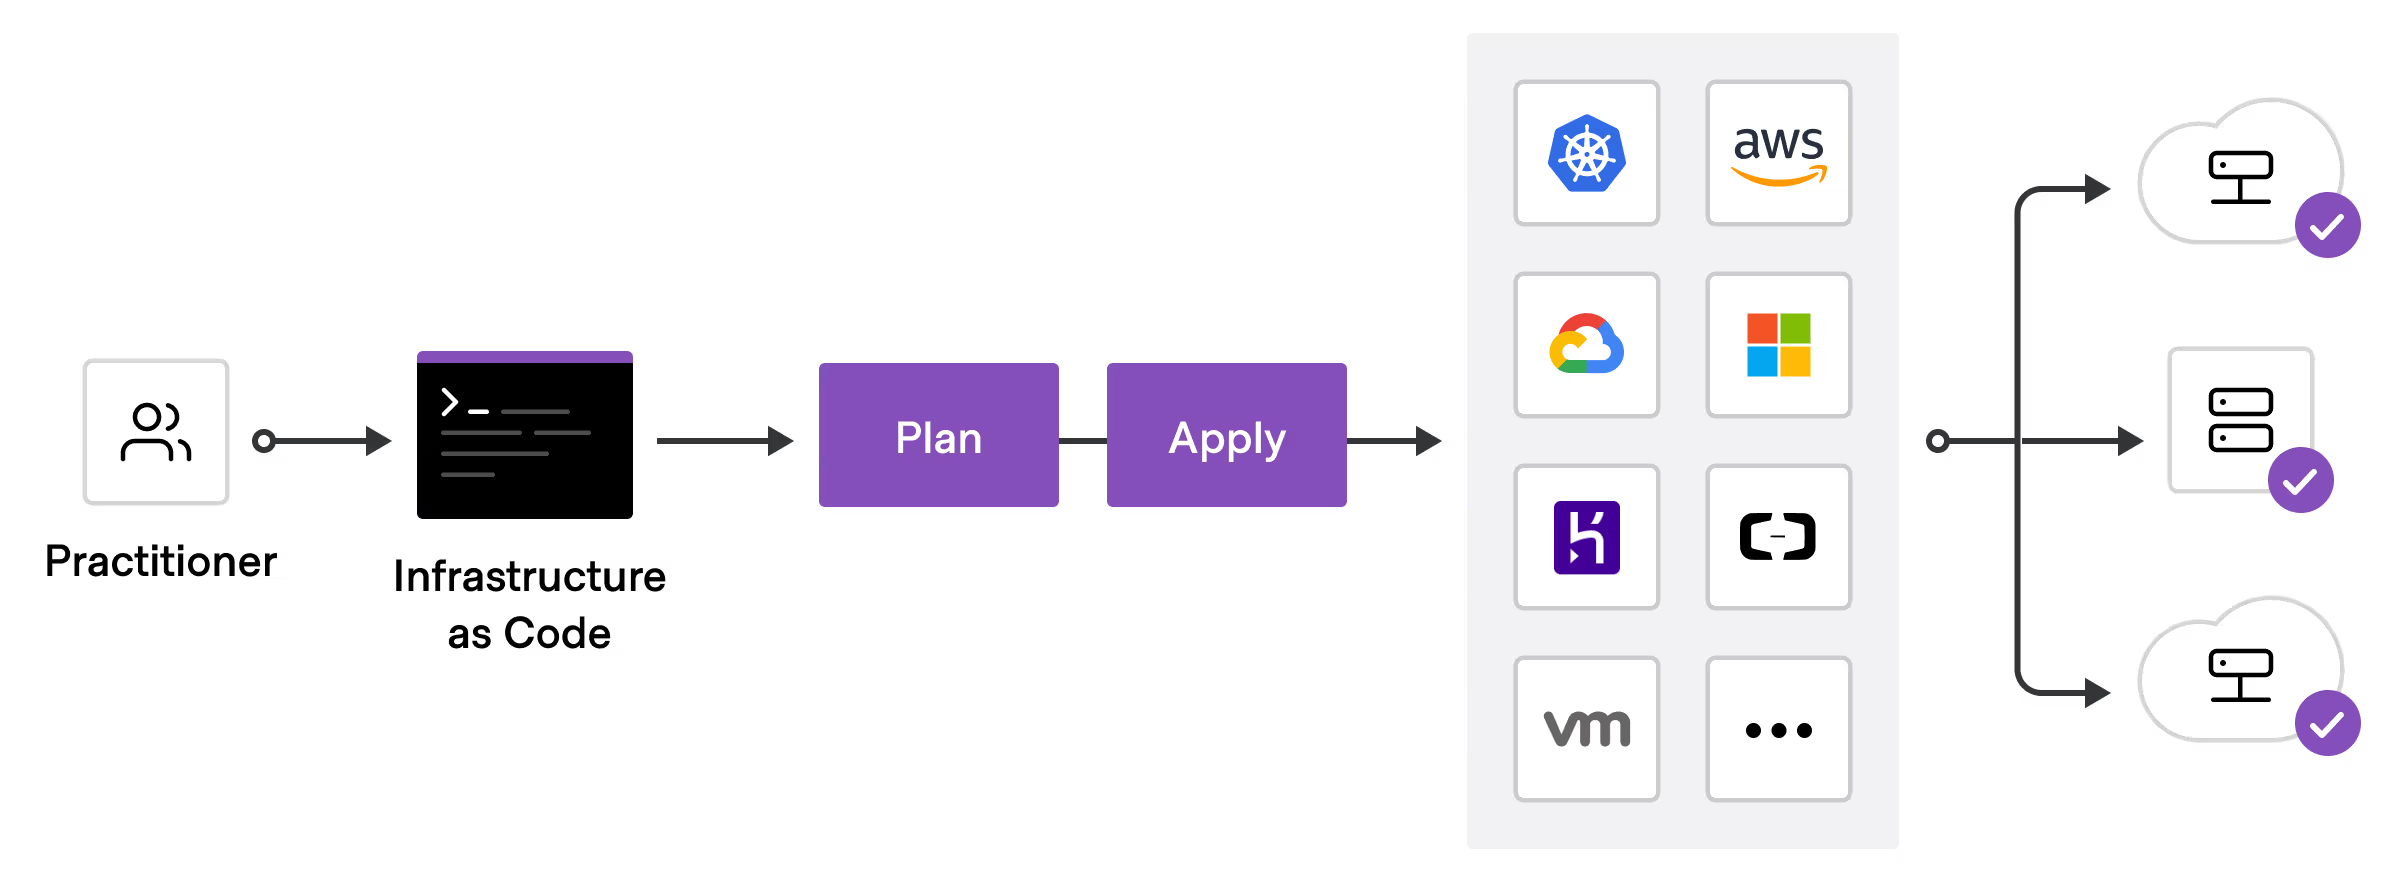
\includegraphics[width=150mm]{assets.png}}
  \caption{Terraform process flow}
  \label{img:terraform-process-flow}
\end{figure}

To deploy infrastructure with Terraform(\ref{img:terraform-process-flow}):

\begin{itemize}
  \item {\textbf{Scope}: Identify the infrastructure for your project.}
  \item {\textbf{Author}: Write the configuration for your infrastructure.}
  \item {\textbf{Initialize}: Install the plugins Terraform needs to manage the infrastructure.}
  \item {\textbf{Plan}: Preview the changes Terraform will make to match your configuration.}
  \item {\textbf{Apply}: Make the planned changes.}
\end{itemize}
\section{Track your infrastructure}
Terraform keeps track of your real infrastructure in a state file, which acts as a source of truth for your environment.
Terraform uses the state file to determine the changes to make to your infrastructure so that it will match your configuration.

\begin{lstlisting}[caption=terraform.tf,language=Terraform]
  terraform {
    required_providers {
      docker = {
        source  = "kreuzwerker/docker"
        version = "~> 3.0.2"
      }
    }
    required_version = "~> 1.7"
  }
\end{lstlisting}

This file includes the terraform block, which defines the provider and Terraform versions you will use with this project.

\begin{lstlisting}[caption=main.tf,language=Terraform]
  provider "docker" {}

  resource "docker_image" "nginx" {
    name         = "nginx:latest"
    keep_locally = false
  }

  resource "docker_container" "nginx" {
    image = docker_image.nginx.image_id
    name  = "tutorial"
    ports {
      internal = 80
      external = 8000
    }
  }
\end{lstlisting}

\begin{lstlisting}[language=bash]
  terraform init
\end{lstlisting}

Provision the NGINX server container with apply. When Terraform asks you to confirm, type yes and press ENTER.

\begin{lstlisting}[language=bash]
  terraform apply
\end{lstlisting}

Run \lstinline{docker ps} to view the NGINX container running in Docker via Terraform.

\begin{lstlisting}[language=bash]
  docker ps
\end{lstlisting}

\begin{lstlisting}[language=bash]
  terraform destroy
\end{lstlisting}
To stop the container and destroy the resources created in this tutorial, run \lstinline{terraform destroy}. When Terraform asks you to confirm, type yes and press ENTER.

\section{CLI Usage} 

Create a directory named \lstinline{learn-terraform-docker-container}.
\begin{lstlisting}[language=bash]
  mkdir learn-terraform-docker-container
\end{lstlisting}

This working directory houses the configuration files that you write to describe the infrastructure you want Terraform to create and manage.
When you initialize and apply the configuration here, Terraform uses this directory to store required plugins, modules (pre-written configurations), and information about the real infrastructure it created.
Navigate into the working directory.

\begin{lstlisting}[language=bash]
  cd learn-terraform-docker-container
\end{lstlisting}
In the working directory, create a file called \href{run:../resources/learn-terraform-docker-container/main.tf}{main.tf} and paste the following Terraform configuration into it.
\begin{lstlisting}[language=Terraform, caption={main.tf}]

  terraform {
    required_providers {
      docker = {
        source  = "kreuzwerker/docker"
        version = "~> 3.0.1"
      }
    }
  }

  provider "docker" {
    # remove host for mac or linux
    host    = "npipe:////.//pipe//docker_engine"
  }

  resource "docker_image" "nginx" {
    name         = "nginx"
    keep_locally = false
  }

  resource "docker_container" "nginx" {
    image = docker_image.nginx.image_id
    name  = "tutorial"

    ports {
      internal = 80
      external = 8000
    }
  }
\end{lstlisting}
Initialize the project, which downloads a plugin called a provider that lets Terraform interact with Docker.

\begin{lstlisting}[language=bash]
  terraform init
\end{lstlisting}
Provision the NGINX server container with apply. When Terraform asks you to confirm type yes and press ENTER.
\begin{lstlisting}[language=bash]
  terraform apply
\end{lstlisting}
Verify the existence of the NGINX container by visiting \url{localhost:8000} in your web browser or running \lstinline{docker ps} to see the container.
To stop the container, run terraform destroy.
\begin{lstlisting}[language=bash]
  terraform destroy
\end{lstlisting}
You've now provisioned and destroyed an NGINX webserver with Terraform.

\section{Build infrastructure}
Deploy a \acrfull{vcn} on \acrfull{oci} using Terraform. Other \acrshort{oci} resources need to deploy into a VCN.
\subsection{Prerequisites}
\begin{enumerate}
  \item{\href{https://docs.oracle.com/en/cloud/foundation/cloud_architecture/governance/tenancy.html}{\acrshort{oci} Tenancy}}
  \item{The Terraform \acrfull{cli} installed.}
  \item{The \acrshort{oci} \acrshort{cli} installed.}
\end{enumerate}


\begin{lstlisting}[language=bash, caption={Configure the OCI CLI from your terminal}, label={lst:configure-the-oci-cli-from-your-terminal}]
  oci session authenticate
  # Enter a region by index or name(e.g.
  # 1: ap-chiyoda-1, 2: ap-chuncheon-1, 3: ap-hyderabad-1, 4: ap-melbourne-1, 5: ap-mumbai-1,
  # 6: ap-osaka-1, 7: ap-seoul-1, 8: ap-sydney-1, 9: ap-tokyo-1, 10: ca-montreal-1,
  # 11: ca-toronto-1, 12: eu-amsterdam-1, 13: eu-frankfurt-1, 14: eu-zurich-1, 15: me-dubai-1,
  # 16: me-jeddah-1, 17: sa-santiago-1, 18: sa-saopaulo-1, 19: uk-cardiff-1, 20: uk-gov-cardiff-1,
  # 21: uk-gov-london-1, 22: uk-london-1, 23: us-ashburn-1, 24: us-gov-ashburn-1, 25: us-gov-chicago-1,
  # 26: us-gov-phoenix-1, 27: us-langley-1, 28: us-luke-1, 29: us-phoenix-1, 30: us-sanjose-1):
\end{lstlisting}

Follow the prompts to enter the region where you have \acrshort{oci} tenancy. A browser window automatically opens and prompts you for your \acrshort{oci} user name and password. Enter them and click the "Sign In" button. Then return to your terminal. It displays a success message, which means that you have configured the \acrshort{oci} \acrshort{cli} with a default profile.

\begin{lstlisting}[language=bash]
  oci session authenticate
  # Enter a region by index or name(e.g.
  # 1: ap-chiyoda-1, 2: ap-chuncheon-1, 3: ap-hyderabad-1, 4: ap-melbourne-1, 5: ap-mumbai-1,
  # 6: ap-osaka-1, 7: ap-seoul-1, 8: ap-sydney-1, 9: ap-tokyo-1, 10: ca-montreal-1,
  # 11: ca-toronto-1, 12: eu-amsterdam-1, 13: eu-frankfurt-1, 14: eu-zurich-1, 15: me-dubai-1,
  # 16: me-jeddah-1, 17: sa-santiago-1, 18: sa-saopaulo-1, 19: uk-cardiff-1, 20: uk-gov-cardiff-1,
  # 21: uk-gov-london-1, 22: uk-london-1, 23: us-ashburn-1, 24: us-gov-ashburn-1, 25: us-gov-chicago-1,
  # 26: us-gov-phoenix-1, 27: us-langley-1, 28: us-luke-1, 29: us-phoenix-1, 30: us-sanjose-1):
\end{lstlisting}

Follow the prompts to enter the region where you have \acrshort{oci} tenancy. A browser window automatically opens and prompts you for your \acrshort{oci} user name and password. Enter them and click the "Sign In" button. Then return to your terminal. It displays a success message and prompts you for a profile name.
Enter learn-terraform for your profile name.

The output prints the location where the CLI has stored your token. Terraform will automatically detect the token later in the tutorial, and use the credentials there to create infrastructure. The token has a 1-hour Time To Live (TTL). If it expires, refresh it by providing the profile name.
\begin{lstlisting}[language=bash]
  oci session refresh --profile learn-terraform
  # Attempting to refresh token from https://auth.us-sanjose-1.oraclecloud.com/v1/authentication/refresh
  # Successfully refreshed token
\end{lstlisting}

\subsection{Write configuration}
\begin{itemize}
  \item The set of files used to describe infrastructure in Terraform is known as a Terraform configuration.
  \item You will write your first configuration to define a single \acrshort{oci} \acrshort{vcn}.
  \item Each Terraform configuration must be in its own working directory.
  \item Create a directory for your configuration.
\end{itemize}

\begin{lstlisting}[language=bash]
  mkdir learn-terraform-oci
\end{lstlisting}

\begin{lstlisting}[language=bash]
  cd learn-terraform-oci
\end{lstlisting}

\begin{lstlisting}[language=bash]
  touch main.tf
\end{lstlisting}

Open main.tf in your text editor and paste in the configuration below.
\begin{lstlisting}[language=Terraform]
  terraform {
    required_providers {
      oci = {
        source = "oracle/oci"
      }
    }
  }

  provider "oci" {
    region              = "us-sanjose-1"
    auth                = "SecurityToken"
    config_file_profile = "learn-terraform"
  }

  resource "oci_core_vcn" "internal" {
    dns_label      = "internal"
    cidr_block     = "172.16.0.0/20"
    compartment_id = "<your_compartment_OCID_here>"
    display_name   = "My internal VCN"
  }
\end{lstlisting}

Customize the following values:
\begin{itemize}
  \item {\textbf{region} - value should match your \acrshort{oci} region.}
  \item{\textbf{compartment\_id} - value should match your "\acrfull{ocid}" which you can get by clicking on the profile icon in the far top right of the \acrshort{oci} console and selecting "Tenancy: YourUsername" from the dropdown menu.}
\end{itemize}
Save the customized file.
This is a complete configuration that you can deploy with Terraform. In the following sections, we will review each block of this configuration in more detail.

\section{Terraform block}
The "terraform \{\}" block contains Terraform settings, the required providers Terraform will use to provision your infrastructure.
For each provider, the "source" attribute defines an optional "hostname", a "namespace", and the provider "type". Terraform installs providers from the \href{https://registry.terraform.io}{Terraform Registry} by default. 
In this example configuration, the oci provider's source is defined as oracle/oci, which is shorthand for \textbf{registry.terraform.io/oracle/oci}.

You can also set a version constraint for each provider defined in the \lstinline{required_providers} block.
The \lstinline{version} attribute is optional, but we recommend using it to constrain the provider version so that Terraform does not install a version of the provider that does not work with your configuration. 
If you do not specify a provider version, Terraform will automatically download the most recent version during initialization.

More information at \href{https://developer.hashicorp.com/terraform/language/providers/requirements}{provider source documentation}


\section{Providers}
The provider block configures the specified provider, in our case oci. A provider is a plugin that Terraform uses to create and mange your resources.

The \lstinline{config\_file\_profile} attribute in the \acrshort{oci} provider block refers Terraform to the token credentials stored in the file that the \acrshort{oci} \acrshort{cli} created when you configured it. Never hard-code credentials or other secrets in your configuration files. Like other types of code, you may share and manage your Terraform configuration files using source control, so hard-coding secret values can expose them to attackers.

You can use multiple provider blocks in your Terraform configuration to manage resources from different providers. You can even use different providers together. For example, you could pass the \acrfull{ip} address of an \acrshort{oci} instance to a monitoring resource from DataDog.

\section{Resources}
Use resource blocks to define components of your infrastructure. A resource might be a physical or virtual component such as a \acrshort{vcn}, or it can be a logical resource such as a Heroku application.


Resource blocks have two strings before the block: the \textbf{resource type} and the \textbf{resource name}.
In this example, the resource type is "oci\_core\_vcn" and the name is "internal".
The prefix of the type maps to the name of the provider, in this case, oci. 
Together, the resource type and name form Terraform's unique ID for the resource. For example, the ID of your \acrshort{vcn} is "oci\_core\_vcn.internal"

Resource blocks contain arguments which you use to configure the resource. The example configuration contains arguments that set the \acrfull{dns} label, the \acrfull{cidr} block for the \acrshort{vcn}, your \acrshort{ocid}, and the display name.
The \href{https://registry.terraform.io/providers/oracle/oci/latest}{OCI provider documentation} documents the requried and optional arguments for each resource in the \acrshort{oci} provider.

\section{Initialize the directory}
\begin{lstlisting}[language=bash]
  terraform init

  # Initializing the backend...

  # Initializing provider plugins...
  # - Finding latest version of oracle/oci...
  # - Installing oracle/oci v5.7.0...
  # - Installed oracle/oci v5.7.0 (signed by a HashiCorp partner, key ID 1533A49284137CEB)

  # Terraform has created a lock file .terraform.lock.hcl to record the provider
  # selections it made above. Include this file in your version control repository
  # so that Terraform can guarantee to make the same selections by default when
  # you run "terraform init" in the future.

  # Terraform has been successfully initialized!

  # You may now begin working with Terraform. Try running "terraform plan" to see
  # any changes that are required for your infrastructure. All Terraform commands
  # should now work.

  # If you ever set or change modules or backend configuration for Terraform,
  # rerun this command to reinitialize your working directory. If you forget, other
  # commands will detect it and remind you to do so if necessary.
\end{lstlisting}
Terraform downloads the oci provider and installs it in a hidden subdirectory of your current working directory, named .terraform. The terraform init command prints out which version of the provider was installed. Terraform also creates a lock file named .terraform.lock.hcl which specifies the exact provider versions used, so that you can control when you want to update the providers used for your project.

\section{Format and validate the configuration}
We recommend using consistent formatting in all of your configuration files. The terraform fmt command automatically updates configurations in the current directory for readability and consistency.
Format your configuration. Terraform will print out the names of the files it modified, if any. In this case, your configuration file was already formatted correctly, so Terraform won't return any file names.
\begin{lstlisting}[language=bash]
  terraform fmt
\end{lstlisting}
You can also make sure your configuration is syntactically valid and internally consistent by using the terraform validate command.
Validate your configuration. The example configuration provided above is valid, so Terraform will return a success message.
\begin{lstlisting}[language=bash]
  terraform validate
\end{lstlisting}

\section{Create infrastructure}
Apply the configuration now with the terraform apply command.
Terraform will print output similar to what is shown below. 
We have truncated some of the output to save space.

\begin{lstlisting}[language=bash]
  terraform apply

  # Terraform used the selected providers to generate the following execution plan. Resource actions are indicated with the following symbols:
  #   + create
  # 
  # Terraform will perform the following actions:
  # 
  #   # oci_core_vcn.internal will be created
  #   + resource "oci_core_vcn" "internal" {
    #       + byoipv6cidr_blocks               = (known after apply)
    #       + cidr_block                       = "172.16.0.0/20"
    #       + cidr_blocks                      = (known after apply)
    #       + compartment_id                   = "ocid1.tenancy.oc1...."
    #       + default_dhcp_options_id          = (known after apply)
    #       + default_route_table_id           = (known after apply)
    #       + default_security_list_id         = (known after apply)
    #       + defined_tags                     = (known after apply)
    #       + display_name                     = "My internal VCN"
    #       + dns_label                        = "internal"
    #       + freeform_tags                    = (known after apply)
    #       + id                               = (known after apply)
    #       + ipv6cidr_blocks                  = (known after apply)
    #       + ipv6private_cidr_blocks          = (known after apply)
    #       + is_ipv6enabled                   = (known after apply)
    #       + is_oracle_gua_allocation_enabled = (known after apply)
    #       + state                            = (known after apply)
    #       + time_created                     = (known after apply)
    #       + vcn_domain_name                  = (known after apply)
  #     }
  # 
  # Plan: 1 to add, 0 to change, 0 to destroy.
  # 
  # Do you want to perform these actions?
  #   Terraform will perform the actions described above.
  #   Only 'yes' will be accepted to approve.
  # 
  #   Enter a value:
\end{lstlisting}

Before it applies any changes, Terraform prints out the execution plan which describes the actions Terraform will take in order to change your infrastructure to match the configuration.
The output format is similar to the diff format generated by tools such as Git.
The output has a + next to "oci\_core\_vcn.internal", meaning that Terraform will create this resource. Beneath that, it shows the attributes that will be set.
When the value displayd is \(known after apply\), it means that the value won't be known until the resource is created.
For instance, \acrshort{oci} assigns its own ID when it creats the \acrshort{vcn}, so Terraform can't know the value of the ID attribute until you apply the change and the \acrshort{oci} provider returns that vlaue from the \acrshort{oci} \acrfull{api},

Terraform will n2wo pause and wait for you approval before proceeding. If anything int the plan seems incorrect or dangerous, it is safe to abort here with no changes made to you infrastructure.

In this case the plan is acceptable, so type yes at the confirmation prompt to proceed. Executing the plan will take a few minutes since Terraform waits for the \acrshort{vcn} to become available.
You've now created infrastructure using Terraform! Visit the \href{https://cloud.oracle.com/networking/vcns}{OCI console \acrshort{vcn} page}, select your compartment, and find your new \acrshort{vcn}, listed as "My internal VCN".

\section{Inspect State}
When you applied your configuration, Terraform wrote data into a file called terraform.tfstate. Terraform stores the IDs and properties of the resources it manages in this file, so that it can update or destroy those resources going forward.

The Terraform state file is the only way Terraform can track which resources it manages, and often contains sensitive information, so you must store your state file securely and distribute it only to trusted team members who need to manage your infrastructure. In production, we recommend storing your state remotely with \href{https://cloud.hashicorp.com/products/terraform}{HCP Terraform} or Terraform Enterprise. 
Terraform also support servral other \href{https://developer.hashicorp.com/terraform/language/backend}{remote backends} you can use to store and manage your state.

Inspect state using \lstinline{terraform show}
\begin{lstlisting}[language=bash]
  terraform show
  # # oci_core_vcn.internal:
  # resource "oci_core_vcn" "internal" {
    #     cidr_block               = "172.16.0.0/20"
    #     cidr_blocks              = [
    #         "172.16.0.0/20",
    #     ]
    #     compartment_id           = "ocid1.tenancy.oc1...."
    #     default_dhcp_options_id  = "ocid1.dhcpoptions.oc1.us-sanjose-1.aaaaaaaa6odqyurw4mf7jmf3jy6ehtw6n32ohyogy4w5c43qoubgewyxr2va"
    #     default_route_table_id   = "ocid1.routetable.oc1.us-sanjose-1.aaaaaaaan3n6iazjfubarvwwtszl3v6gdzqvfoccdj555p2ujehbo4tlu7ma"
    #     default_security_list_id = "ocid1.securitylist.oc1.us-sanjose-1.aaaaaaaant6vlu2y77pwwzjubmzg6czzvo2laii4h3p5d7w2nqcr4fey5gaa"
    #     defined_tags             = {
      #         "Oracle-Tags.CreatedBy" = "oracleidentitycloudservice/redacted"
      #         "Oracle-Tags.CreatedOn" = "2021-04-07T18:25:06.555Z"
    #     }
    #     display_name             = "My internal VCN"
    #     dns_label                = "internal"
    #     freeform_tags            = {}
    #     id                       = "ocid1.vcn.oc1.us-sanjose-1.amaaaaaapqqlmeyaklull6tpfms534aoijpjwpkzjo25rxqiqhadgdzodnua"
    #     ipv6cidr_blocks          = []
    #     ipv6private_cidr_blocks  = []
    #     is_ipv6enabled           = false
    #     state                    = "AVAILABLE"
    #     time_created             = "2021-04-07 18:25:06.558 +0000 UTC"
    #     vcn_domain_name          = "internal.oraclevcn.com"
  # }
\end{lstlisting}
When Terraform created this \acrfull{vcn}, it also gathered a lot of information about it from the \acrshort{oci} provider. These values can be referenced to configure other resources or outputs.

\section{Manually managing state}
Terraform has a built-in command called terraform state for advanced state management. For example, you may want a list of the resources in your project's state, which you can get by using the list subcommand.

\begin{lstlisting}[language=bash]
  terraform state list
  # oci_core_vcn.internal
\end{lstlisting}

\end{document}
% \begin{lstlisting}[language=Terraform, caption={}, label={lst:}]
% \end{lstlisting}

% \begin{lstlisting}[language=bash, caption={}, label={lst:}]
% \end{lstlisting}
